\documentclass[a4paper]{article}
\usepackage[left=2cm,right=2cm]{geometry}
\usepackage{amsmath}
\usepackage[dvipsnames]{xcolor}
\usepackage{graphicx}
\usepackage{latexsym}
\usepackage{amsfonts}
\usepackage{amssymb}
\usepackage{wasysym}
\usepackage{multirow}

% shortcut for \texttt 
\newcommand{\cd}{\texttt}
% double backslash - used in MathGL syntax
\newcommand{\dbs}{\textbackslash\textbackslash}

\begin{document}
\begin{center}
Plotting in 1-D 
\begin{tabular}{l|l}
  \textsc{Matlab} & MathGL \\
  \hline\hline
  \cd{axis([0,5,-2,2])} & \cd{gr.Ranges(0,5,-2,2)} \\
  Default: autofit (\cd{axis \textcolor{Orchid}{auto}}) & Default: \cd{x=-1:1}, \cd{y=-1:1} \\
                                                        & Workaround: \cd{gr.Ranges(x.Minimal(), x.Maximal(),} \\
                                                        & \cd{y.Minimal(), y.Maximal())} \\
  \hline
  \cd{axis([0,5,-inf,inf])} & \cd{gr.Range('x',0,5)} \\
  \hline
  \cd{axis([-inf,inf,-2,2])} & \cd{gr.Range('y',-2,2)} \\
  \hline
  \cd{xlabel('x-axis')} & \cd{gr.Label('x', "x-axis")} \\
  \hline
  \cd{ylabel('y-axis')} & \cd{gr.Label('y', "y-axis")} \\
  \hline
  \multirow{3}{15em}{\cd{legend('sin(x)', 'x\^{}2')}}& \cd{gr.AddLegend("sin(x)","b")} \\
                                                     & \cd{gr.AddLegend("\dbs x\^{}2", "g")} \\
                                                     & \cd{gr.Legend()} \\
  \hline
  \cd{legend('exp(x)')} & \cd{gr.AddLegend("exp(x)","b")} \\
  \cd{legend('boxoff')} & \cd{gr.Legend(1,1,"")} \\
  \hline
  \multirow{2}{20em}{\cd{legend('x','Location','northwest')}}  & \cd{gr.AddLegend("x","b")} \\
                                                               & \cd{gr.Legend(0,1)} \\
  \hline
  \multirow{2}{20em}{\cd{legend('cos(x)', 'Orientation', 'horizontal')}} & \cd{gr.AddLegend("cos(x)","b")} \\
                                                                        & \cd{gr.Legend("\#-")} \\
  \hline
  \multicolumn{2}{l}{
    \begin{minipage}{5cm}
      $ \begin{vmatrix}
    (0,1) & (0.5, 1) & (1,1) \\
    (0,0.5) & (0.5,0.5) & (1,0.5) \\
    (0,0) & (0.5,0) & (1,0)
      \end{vmatrix} $
    \end{minipage}
    \hfill
    \begin{minipage}{10cm}
      Legend alignment in MathGL: \\
      Values larger than 1 will give position outside of the graph. \\
      Default is (1,1).
    \end{minipage}
  } \\

  \hline
  \cd{plot(y)} & \cd{gr.Plot(y)} \\
  \hline
  \cd{plot(t,y)} & \cd{gr.Plot(t,y)} \\
  \hline
  \multirow{2}{15em}{\cd{plot(t0,y0,t1,y1)}} & \cd{gr.Plot(t0,y0)} \\
                                            & \cd{gr.Plot(t1,y1)} \\
  \cd{plot(t,y,'b+')} & \cd{gr.Plot(t,y,"b+")} \\
  \hline
  \multicolumn{2}{l}{Possible linestyles and linecolors: see follwing tables.} \\
  \hline
  \cd{print('myfig','-depsc')} & \cd{gr.WriteEPS("myfig.eps")} \\
  \cd{print('myfig','-dpng')} & \cd{gr.WritePNG("myfig.png")} (compile w/ flag \cd{-lpng}) \\
  \hline
  \multirow{2}{15em}{\cd{title('Plot title')}}  & \cd{gr.Title("Plot title")} (title high above plot) \\
                                                &$\left.\begin{array}{c}
                                                    \text{\cd{gr.Subplot(1,1,0,"<\_")}} \\
                                                    \text{\cd{gr.Title("Plot title")}}
                                                  \end{array} \right\}$
                                                    (title directly above plot) \\


  


\end{tabular}
\end{center}

\begin{center}
Plotting in 2-D

\begin{tabular}{l|l}
  \textsc{Matlab} & MathGL \\
  \hline\hline
  \cd{colorbar} & \cd{gr.Colorbar()} \\
  \hline
  \cd{mesh(Z)} & \cd{gr.Mesh(Z)} \\ 
  \cd{mesh(X,Y,Z)} & \cd{gr.Mesh(X,Y,Z)} \\
  \hline
  \cd{surface(Z)} & \cd{gr.Surf(Z)} \\ 
  \cd{surface(X,Y,Z)} & \cd{gr.Surf(X,Y,Z)} \\
  \hline
  \cd{pcolor(Z)} & \cd{gr.Tile(Z)} \\ 
  \cd{pcolor(X,Y,Z)} & \cd{gr.Tile(X,Y,Z)} \\
  \hline
  \cd{plot3(X,Y,Z)} & \cd{gr.Plot(X,Y,Z)} \\
\end{tabular} 
\end{center}
Additionaly you have to add \cd{gr.Rotate(50,60)} before the plot command for MathGL to create a 3-D box,
otherwise the result is 2-D.


\begin{minipage}{3cm}
  Linecolors\footnote{
  Upper-case letters will give a darker version of the lower-case version.
  }:\\ \\
  \begin{tabular}{l|c}
    \textcolor{blue}{blue} & \cd{b} \\
    \textcolor{green}{green} & \cd{g} \\
    \textcolor{red}{red} & \cd{r} \\
    \textcolor{cyan}{cyan} & \cd{c} \\
    \textcolor{magenta}{magenta} & \cd{m} \\
    \textcolor{yellow}{yellow} & \cd{y} \\
    \textcolor[gray]{0.5}{gray} & \cd{h} \\
    \textcolor{SeaGreen}{green-blue} & \cd{l} \\
    \textcolor{RoyalBlue}{sky-blue} & \cd{n} \\
    \textcolor{orange}{orange} & \cd{q} \\
    \textcolor{LimeGreen}{green-yellow} & \cd{e} \\
    \textcolor{CadetBlue}{blue-violet} & \cd{u} \\
    \textcolor{purple}{purple} & \cd{p}
  \end{tabular}
\end{minipage}
\hfill
\begin{minipage}{3cm}
  Linestyles:\\ \\
  \begin{tabular}{l|c}
    solid & \cd{-} \\
    dashed & \cd{;} \\
    small dashed & \cd{=} \\
    long dashed & \cd{|} \\
    dotted & \cd{:} \\
    dash-dotted & \cd{j} \\
    small dash-dotted & \cd{i} 
  \end{tabular}
\end{minipage}
\hfill
\begin{minipage}{3cm}
  Linemarkers:\\ \\
  \begin{tabular}{l|c}
    + & \cd{+} \\
    o & \cd{o} \\
    $\diamond$ & \cd{d} \\
    $\cdot$ & \cd{.} \\
    $\triangle$ & \cd{\^{}} \\
    $\nabla$ &\cd{v} \\
    $\lhd$ & \cd{<} \\
    $\rhd$ & \cd{>} \\
    $\odot$ & \cd{\#.} \\
    $\boxplus$ & \cd{\#+} \\
    $\boxtimes$ & \cd{\#x} 
  \end{tabular}
\end{minipage}

\begin{center}
  Fonts
\end{center}

\begin{figure}[h]
  \begin{minipage}{7cm}
     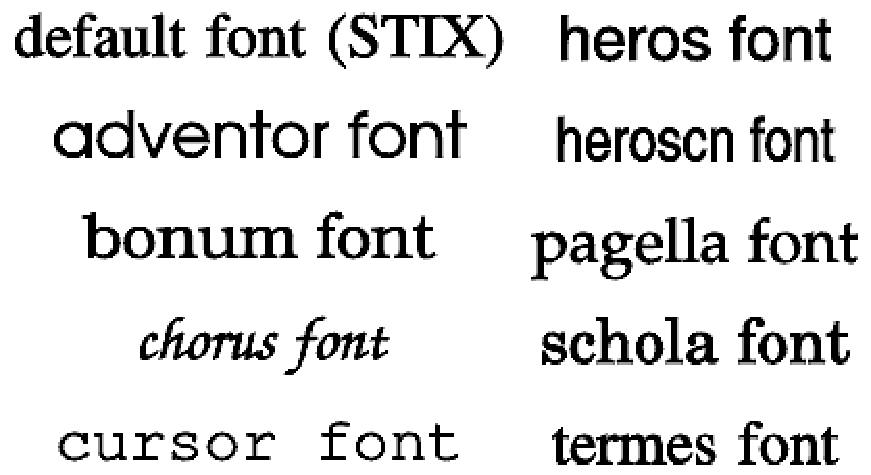
\includegraphics[width=1\textwidth]{font-families.pdf}
     \caption{\cd{gr.SetFont("scholar")} will set the font to ``scholar''}
  \end{minipage}
    \hfill
  \begin{minipage}{9cm}
  \begin{center}Font sizes\end{center}
    \cd{gr.SetFontSizePT(12)} sets the font size to 12pt \\
    \cd{gr.SetFontSizeCM(0.5)} sets the font size to 0.5cm \\
    \cd{gr.SetFontSizeIN(0.22)} sets the font size to 0.22 inch \\
    In-Line changes and indices: \\
    \cd{gr.Title("@\{center-index\}")} in smaller size \\
    \cd{gr.Title("\_\{lower-index\}")} in tiny size \\
    \cd{gr.Title("\^{}\{upper-index\}")} in tiny size \\
    \cd{gr.Title("\dbs big\{Large\}")} in larger size \\
    All sizes here are relative to the default sizes. 
    E.g.: \cd{big} in the Title is larger than in other places. \\ 
  \end{minipage}
\end{figure}

\end{document}
